\documentclass[11pt,a4paper]{article}


\usepackage{amssymb,amsmath,amsfonts}    %ams
\usepackage{wasysym} %des symboles
%\usepackage{a4wide}
\usepackage[tmargin=1in,bmargin=1in,lmargin=.75in,rmargin=.75in]{geometry}
\usepackage{graphicx}
%\usepackage{pstricks}
%\usepackage{multido}
\usepackage{verbatim}
\usepackage{enumerate}
\usepackage{tikz}
\usetikzlibrary{calc,positioning,backgrounds}

\usepackage[utf8]{inputenc} 
%\usepackage[T1]{fontenc}
\usepackage{listings}

\newcommand{\R}{{\mathbb R}}   % reals
\newcommand{\Q}{{\mathbb Q}}   % rationals
\newcommand{\N}{{\mathbb N}}   %natural numbers
\newcommand{\Z}{{\mathbb Z}}    %integers
\renewcommand{\P}{{\mathbb P}}   %primes
\newcommand{\F}{{\mathbb F}}

\newcommand\cc{{\cal C}}
\newcommand{\cw}{{\cal W}}



\newtheorem{theorem}{Theorem}
\newtheorem{cor}{Corollary}
\newtheorem{example}{Example}
\newtheorem{lemma}{Lemma}
\newtheorem{newcommandi}{Definition}


\newcommand{\proof}{\noindent {\bf Proof.\ \ }}

\newcommand{\qed}{\hfill $\square$}


\newcommand{\card}[1]{\vert #1 \vert}

%\newcommand{\qed}{\hspace*{\fill} $\Box$ \bigskip }


%\renewcommand{\thefootnote}{\Alph{footnote}}
\usepackage{fancybox}
\usepackage[french]{babel}
%\usepackage{fullpage}
\usepackage{multicol}
\setlength{\columnseprule}{0.2pt}
\setlength{\columnsep}{16pt}
\usepackage{fancyhdr} % personalisation tete/pied de page
%\pagestyle{fancy}







\usepackage{hyperref}

%\addtolength{\headheight}{50pt}

\setlength{\parindent}{0pt}

\title{Fiche 4.0 : récursivité}
\author{BUT Informatique\\
IUT de Vélizy\\
}
\date{}


%\catcode`\_=12 %for escaping underscore

\newcommand{\ww}[1]{\textcolor{white}{#1}}

\newcommand{\code}[1]{%
    \begin{center}
        \tt #1
        \vskip .2cm
        {\tt
            \lstinputlisting[frame=single]{#1}
        }
    \end{center}
}


\usepackage{marginnote}

\usepackage{fancyvrb} % Verbatim avancé

\lstdefinestyle{customc}{
    belowcaptionskip=1\baselineskip,
    breaklines=true,
    frame=single,
    xleftmargin=2cm,
    language=C,
    showstringspaces=false,
    showspaces=false,
    basicstyle=\ttfamily
}


\newcommand{\reflexion}{\hspace{-1.2cm} 
\includegraphics[width=1cm]{reflexion.jpg} \vskip -.8cm}
%\newcommand{\checkbox}{
\includegraphics[width=.5cm]{checkbox.jpg} }
\newcommand{\checkbox}{$\square$ \smallskip}


%%environement pour les icones avec decalage
\newenvironment{icone}[1]{%
    \hskip -.8cm
\begin{tabular}{c|c}
    \hspace{.03\textwidth} \includegraphics[width=.07\textwidth]{#1} & 
\begin{minipage}{.85\textwidth}
}{%
\end{minipage}
\end{tabular}
}





\newcounter{exo} \setcounter{exo}{0}
\newenvironment{action}{%
    \begin{enumerate}[\numerotation] \addtocounter{exo}{-1}%
        }{%
    \end{enumerate}
}

%environement pour liste avec checkbox avec compteur
\newcommand{\numexoa}{\theexo \addtocounter{exo}{1}}
\newcommand{\numerotation}{\checkbox \smallskip \numexoa.}

%%environement de validation
\newenvironment{validation}{%
\smallskip
\begin{tabular}{c|c}
    \hspace{.03\textwidth} 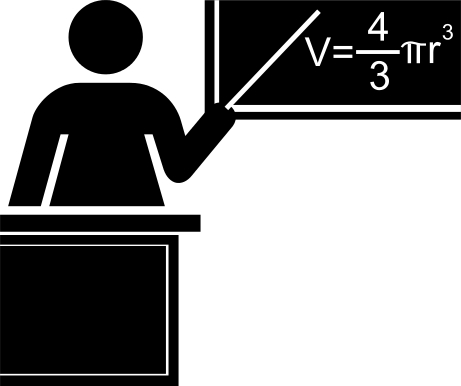
\includegraphics[width=.07\textwidth]{teacher.jpg} & 
\begin{minipage}{.85\textwidth}
}{%
\end{minipage}\\
\hline
\end{tabular}
}


%pour les fichiers c et dossiers
\newcounter{exoo} \setcounter{exoo}{0}
\newcommand{\numexo}{\theexoo}
\newcommand{\repexo}{{\tt exo\_\numexo}}
\newcommand{\exoplus}{\addtocounter{exoo}{1}}




\begin{document}
\maketitle





\thispagestyle{empty}

\setcounter{section}{-1}
\section{Empilements}

\begin{action}
\item {\bf Prise en main - \tt empilements0.} Lisez le code et exécutez-le. Cet exercice utilise une mini-bibliothèque {\tt libEmpilements} 
qui étend {\tt tkiteasy} ; les exercices qui suivent seront faits sur le même modèle.
L'objectif de cette question est seulement de comprendre l'utilisation de la méthode {\tt empilerCube}. 
Modifiez librement le script en ajoutant des cubes supplémentaires empilés avec les premiers ou sur des espaces vides.
\item {\bf Trois fonctions - \tt empilements1.} Ce script définit trois fonctions qui s'appellent entre elles. L'objectif ici
est de comprendre en regardant le code pourquoi les cubes tombent exactement dans cet ordre et sur ces positions.
\item {\bf Sans tricher ! - \tt empilements2.} Si vous avez compris, essayez de prévoir 
dans quel ordre et à quels endroits vont tomber les cubes si l'on fait l'appel de fonction {\tt fa(g,2)} (il faut l'ajouter). Prenez un papier et essayez
de noter dans quel ordre tombent les cubes, sur quel emplacement et avec quelle couleur ! Si vous vous êtes trompé, 
ce n'est pas grave mais essayez de comprendre pourquoi !
\item {\bf Cette fois-ci, vraiment sans tricher ! - \tt empilements3.} Même exercice si l'on ajoute dans ce script l'appel de fonction {\tt fA(g,2)}.
\item {\bf Chassé-croisé - \tt empilements4.}  Essayez de prévoir ce que va faire l'appel {\tt f0(g,0)}.
\item {\bf suite - \tt empilements4.} A la fin de la fonction {\tt f0}, ajoutez l'empilement d'un cube rouge sur la même
position que le cube bleu. Comment et dans quel ordre cela va-t'il se passer ?
\item {\bf Valideycheun} Appelez l'enseignant.e afin de valider ce que vous avez compris des 4 exercices précédents.
\end{action}

\begin{icone}{img/lecture.jpg}
  Dans l'exercice précédent, vous avez vu deux fonctions {\tt f0} et {\tt f1} qui s'appellent l'une l'autre. Il ne nous
  reste plus beaucoup de chemin à faire pour utiliser maintenant une fonction qui s'appelle elle-même : une fonction {\it récursive}.

  Attention : dans les exercices ci-dessous, celle ou celui qui écrit une boucle va au coin !
\end{icone}


\begin{action}
\item {\bf Première fonction récursive - \tt empilements5}. La fonction qui effectue le travail d'empilement de cubes est la fonction {\tt f0}. 
Comme vous le voyez cette fonction ne contient pas de boucle.  La ligne où la fonction {\tt f0}
appelle la fonction {\tt f0} dans son propre code est \emph{l'appel récursif}. 
\item {\bf Suite - \tt empilements5}. Déplacez l'appel récursif \emph{avant} l'empilement. Que se passe-til ? Expliquez !
\item {\bf Suite - \tt empilements5}. Modifiez le code afin d'empiler un cube bleu de gauche à droite, puis un cube vert
de droite à gauche, avec un seul appel récursif !
\item {\bf A vous - \tt empilements6}. Sur le modèle de l'exercice précédent, écrivez une fonction récursive mais qui
fasse une récurrence descendante, de la position 9 à la position 0 en empilant des cubes. Puis modifiez le code afin
d'obtenir un empilement de droite à gauche, suivi d'une seconde ligne de gauche à droite (toujours un seul appel récursif.)
\item {\bf remplissage - \tt empilements7 } La fonction {\tt f0} de l'exercice précédent, dans sa première version permettait de remplir
toute une ligne. Pouvez-vous créer une deuxième fonction qui va appeler {\tt f0} pour remplir une ligne, 
puis qui va s'appeler elle-même afin de remplir la ligne du-dessus ? Si cela fonctionne, tout l'écran sera rempli par récurrence.
Attention, il faut s'arrêter à un moment quand les lignes deviennent trop hautes (vous pouvez avoir besoin d'un compteur passé en paramètre).
\end{action}


\section{Exploration-Diffusion}

Dans ce nouvel environnement graphique, nous allons étudier le concept de diffusion ou d'exploration, 
qui consiste en général à partir d'un endroit précis et d'explorer de proche en proche tous les endroits accessibles.


\begin{action}
\item {\bf démonstration - \tt demo\_grille1.mp4} visualiser le film {\tt demo\_grille1.mp4} afin de voir concrètement l'objectif de cette partie.
\end{action}
\begin{icone}{img/lecture.jpg}
Il s'agit d'une version préliminaire des algorithmes de plus court chemin. Dans cette version, Pacman se trouve dans un environnement 2D
où il peut se déplacer dans 4 directions, et ne peut pas traverser les murs (cases noires). L'objectif est de déterminer l'ensemble
des cases auxquelles Pacman peut accéder, en visualisant de plus les appels récursifs par des flèches.
\end{icone}



\begin{action}
\item {\bf tuto de l'API - \tt grille0.} lisez le code de {\tt grille0.py} et exécutez. Attention surveillez aussi le terminal. Le but
est de comprendre l'interface qui sera utilisée ensuite.
\item {\bf première tentative - \tt grille1} Même chose, sauf qu'ici on fait se déplacer pacman jusqu'à ce qu'il soit coincé.
Essayez de modifier ce code pour que tout se passe comme dans le film {\tt demo\_grille2.py}.
\begin{itemize}
    \item lorsque Pacman se déplace, on marque son déplacement avec une flèche rouge.
    \item lorsque Pacman rencontre un obstacle, il essaie de repartir dans une autre direction. Indication : on peut faire
    {\tt dx, dy = dy, -dx} pour effectuer un quart de tour sur la direction !
    \item Si toutes les directions sont bloquées car soit déjà explorées (couleur "blue") ou invalides, alors le programme se termine.
\end{itemize}
Peut-on faire mieux avec cet algorithme? Réussir à visiter toutes les cases accessibles?
\item {\bf version récursive - \tt grille2} Finalement, la technique ci-dessus a clairement ses limites : Pacman peut se retrouver bloqué et 
il faut trouver le moyen de "repartir en arrière". C'est là qu'intervient la récursivité et la pile d'appels (ou pile de récursivité)
fait ce travail pour nous. Complétez la fonction {\tt exploration} qui se trouve dans le fichier grille2. La spécification de la fonction
donne les instructions à suivre.
\end{action}

\section{Exercices non graphiques}

\begin{icone}{img/lecture.jpg}
  Après le déroulement graphique passionant des deux parties précédentes, vous avez développé une intuition solide
  du déroulement d'une fonction récursive. Les exercices qui suivent, plus classiques, sont à traiter
  dans des scripts python sans sortie graphique (terminal uniquement). Vous pouvez également utiliser {\tt jupyter}.
\end{icone}


\begin{action}
\item Faites tourner ce programme sur papier (ou dans votre tête) et déterminez ce qu'il fait:
\begin{code}
def fx(t, n):
    if n == len(t):
        return 0

    if t[n] == 0:
        return 1+fx(t, n+1)
    else:
        return fx(t, n+1)

l = [5,3,4,2,0,4,2,0,0,1,0,2]
print(fx(l,0))
\end{code}

\item Faites tourner ce programme sur papier (ou dans votre tête) et déterminez ce qu'il fait:
\begin{code}
def fx(t, n, d, f):
    if d>f:
        return False
    
    m = (d+f)//2
    if t[m] == n:
        return True
    elif t[m] > n:
        return fx(t, n, d, m-1)
    else:
        return fx(t, n, m+1, f)

l = [1,4,8,9,12,17,21,25,90]
print(fx(l, 8, 0, len(l)-1))
print(fx(l, 10, 0, len(l)-1))
print(fx(l, 1, 0, len(l)-1))
\end{code}
  
\item
  \'Ecrire une fonction récursive qui renvoie la somme des entiers $0 ^2 + 1^2 +
  \dots + n^2$, l'entier $n$ étant donné en paramètre (sans utiliser de formule).

\item
\'Ecrire une fonction récursive qui renvoie un booléen indiquant si les éléments
d'un tableau d'entier sont tous positifs.\\
On pourra écrire une fonction de prototype {\tt tout\_positif(tab, debut=0)}
et qui renvoie un booléen qui indique si tous les éléments de {\tt tab}
sont positifs depuis l'indice {\tt debut} jusqu'à la fin.

\item
\'Ecrire une fonction récursive qui cherche un élément dans un tableau. Même
principe que pour l'exercice précédent.\\

\item
\'Ecrire une fonction récursive qui cherche un entier dans un tableau {\bf trié} d'entiers
par recherche dichotomique.\\


\item
\'Ecrire une fonction récursive calculant les termes de la suite de Fibonacci 1 1 2 3 5 8 13 21 34 ... Cette fonction est-elle efficace en termes de complexité algorithmique ? Comment l'améliorer ?

\item \'Ecrire une fonction qui génère toutes les chaînes de caractères
de longueur $k$ (par exemple, les mots de passe !) que l'on peut
écrire étant donné une liste de
caractères de la forme {\tt caracteres = ['a','c','x',...]}.

\item (*) \'Ecrire une fonction récursive qui renvoie la liste de toutes les suites
  strictements
  croissantes de longueur $k$ composées d'entiers de $1$ à $n$.

  Exemple : Si $k=3$ et $n=5$ la fonction doit renvoyer (éventuellement dans un
  autre ordre)
  
\[ [[1,2,3], [1,2,4], [1,2,5], [1,3,4], [1,3,5], [1,4,5], [2,3,4], [2,3,5],
  [2,4,5], [3,4,5] ] \]

\end{action}




\end{document}
